\documentclass[11pt,a4paper]{article}

\usepackage[T1]{fontenc}
\usepackage[utf8]{inputenc}
\usepackage[margin=1.1in]{geometry}
\usepackage[expansion=false]{microtype}
\usepackage{amsmath,amssymb,amsthm}
\usepackage{mathtools}
\usepackage{stmaryrd}
\usepackage{tikz}
\usetikzlibrary{arrows.meta,positioning,fit,backgrounds}
\usepackage[hidelinks]{hyperref}
\usepackage{enumitem}

\theoremstyle{definition}
\newtheorem{definition}{Definition}[section]
\newtheorem{condition}[definition]{Condition}
\newtheorem{requirement}[definition]{Requirement}

\theoremstyle{plain}
\newtheorem{proposition}[definition]{Proposition}
\newtheorem{observation}[definition]{Observation}
\newtheorem{conjecture}[definition]{Conjecture}

\theoremstyle{remark}
\newtheorem{remark}[definition]{Remark}
\newtheorem{question}{Question}

\newcommand{\rc}{\textup{rho}}
\newcommand{\RHO}{\mathsf{RHO}}
\newcommand{\Bee}{\mathcal{B}}
\newcommand{\Cat}{\mathbf{C}}
\newcommand{\quo}[1]{@#1}
\newcommand{\bisim}{\approx}
\newcommand{\sbisim}{\sim}
\newcommand{\Qs}{Q_{\sigma}}

\title{\textbf{Getting the Distribution Is Not Getting the Correspondence}\\[0.4em]
\large Notation, bisimulation, and the bootstrap problem for grounded symbol systems}
\author{}
\date{6 August 2026}

\begin{document}
\maketitle

\begin{abstract}
\noindent A language model trained to predict the next token inherits a correspondence
between symbols and world that it did not construct and cannot inspect. That
correspondence was bootstrapped by the human agents who use the language, and it lives
in them, not in the text. Undeciphered scripts make the point sharply: we possess the
distribution and lack the correspondence, and no amount of the former yields the latter.
The current work on sperm whale codas supplies the complementary control: no cognates, no
anchor language, and decoding is nonetheless thought feasible---because the population is
alive and can be watched using its symbols while it acts. Those same two species are the
proof that the problem is soluble: it has been solved twice, independently, and the two
solutions share three features---a population rather than an individual, an interface that
co-evolved with the symbols rather than being chosen, and a criterion external to the
symbol system---which constrain the shape of any third.
This note lays out the resulting bootstrap problem, provisionally adopts Nelson
Goodman's theory of notationality as an answer to the prior question of what a symbol
system \emph{is}, records where that theory agrees with a bisimulation-based account of
symbol identity and where it demands strictly more, and examines the flexibility of the
reflective higher-order calculus to admit builtin processes drawn from a host world.
Quotation and dereference in the pure calculus turn out to be recursive score
construction rather than a score / performance relation; adjoining builtins is precisely
what re-types them into one. That extension is developed as far as a calculus-making
functor $\RHO[\Bee]$ and then
deliberately halted: it is offered as a suggestive analogy for what a grounded symbol
system would have to look like, not as a solution to the problem of acquiring one. The
note closes with an inventory of open questions, several of which appear tractable.
\end{abstract}

\section{Introduction}

This note is a framing document. It does not report a result; it tries to state a
problem precisely enough that results become possible, and to say honestly which of the
apparatus already in hand bears on it and which does not.

The occasion is a distinction that has become easy to lose. Transformer networks are
applied to two quite different tasks under one description. In the first, the network is
a \emph{transducer}: it receives sensor data and must produce symbols. In the second, it
is a \emph{next-token predictor}: it receives symbols and must produce more of them. The
second task looks like the first performed at scale, and much of the current discourse
treats it that way. It is not. In the second case the transduction has already happened,
performed over millennia by a population of human agents, and the network is working
downstream of a correspondence it neither built nor has access to.

The argument runs in four movements.

\begin{enumerate}[label=(\arabic*),leftmargin=2.2em]
\item \textbf{The problem} (\S\ref{sec:problem}). A living language exists inside a
correspondence between language and environment, and that correspondence is a fact about
the agents, not about the language. Linear A and Rongorongo are the controlled
experiment: the distribution survives, the correspondence does not, and the distribution
does not recover it.
\item \textbf{The proposal} (\S\ref{sec:goodman}). We provisionally adopt Goodman's
notationality as an account of what a symbol system is. It does not solve the bootstrap
problem. It says what would count as having solved it, which is a different and
prerequisite service.
\item \textbf{The fit} (\S\ref{sec:bisim}). Goodman's conditions align closely with a
bisimulation-based treatment of symbol identity, and we say exactly where. Two of his
five conditions are quotient conditions that bisimulation supplies. Two are separation
conditions that it does not. The gap is the interesting part.
\item \textbf{The analogy} (\S\ref{sec:rho}). In the reflective higher-order calculus,
quotation and dereference are mutually inverse but purely score-internal: they witness a
faithful recursion inside the notation, with no performance in the picture. Adjoining
builtin processes from a host world re-types those same operators into a score /
performance correspondence. Read as a calculus-making functor, the extension exhibits
several of Goodman's conditions as structural properties. We develop the reading and
then argue explicitly why it is an analogy and not a solution.
\end{enumerate}

\noindent Open questions are collected in \S\ref{sec:open}, and \S\ref{sec:claims}
separates what is claimed here from what is not.

\paragraph{Relation to the other notes.} This note is a sibling of \emph{The Mortal
Scientist} and \emph{Learning to Play}, and depends on \emph{Composing Learners} for the
argument of \S\ref{sec:social}. Its relation to those notes is adversarial in a
productive way: it identifies a problem the mortal-scientist framework does not face,
explains why it does not face it, and asks what would have to change for it to.

\section{The problem}
\label{sec:problem}

\subsection{A language presupposes a correspondence it does not contain}

Consider what a competent speaker has that a corpus does not. The speaker can be handed
an object and asked whether it is a coconut. The corpus cannot. The speaker's competence
includes a set of dispositions connecting expressions to features of an environment
accessible to the speaker; the corpus records only the traces those dispositions leave in
speech. Harnad's diagnosis remains the clearest: symbolic representations must be
grounded in nonsymbolic ones---iconic representations that are analogues of sensory
projections, and categorical representations that pick out invariants---and elementary
symbols are the names of the categories so picked out \cite{harnad1990}. The names are
recoverable from text. The categories are not.

Bender and Koller's octopus makes the same point as a thought experiment, and Bisk et
al.\ generalise it into a hierarchy of ``world scopes'' along which a text-only system
occupies the narrowest rung \cite{benderkoller2020,bisk2020}. Both are usually read as
arguments about \emph{understanding}, which invites the reply that understanding is
underdefined. We take the sharper reading, which is not about understanding at all: the
correspondence is a physical relation between agent and environment, it is a fact about
the agent, and text is downstream of it. Whether or not anything deserves to be called
understanding, the correspondence is either instantiated somewhere or it is not.

\begin{observation}[The locus of correspondence]
\label{obs:locus}
For a living language $L$ used by a population $A$ in an environment $E$, the
correspondence $c : L \to E$ is realised in $A$. The corpus is the image of
language use under $c$'s having already been applied; it does not contain $c$.
\end{observation}

\noindent The observation is trivial when stated. Its force is that the loss of $A$
destroys $c$ while leaving the corpus intact, and that this is not a hypothetical.

\subsection{The evidence: undeciphered scripts}
\label{sec:decipherment}

The undeciphered scripts are the controlled experiment for
Observation~\ref{obs:locus}. Rongorongo and Linear A are corpora without populations. We
have the marks. We can compute over them. We do not have the correspondence, and
centuries of effort have not manufactured one from the marks alone.

The machine-learning record is unusually informative here, because it isolates the
variable. Luo, Cao and Barzilay's neural decipherment recovers a substantial fraction of
Linear B cognates and improves the state of the art on Ugaritic \cite{luo2019}. The
method works because Linear B was already known to encode an early form of Greek and
Ugaritic an early form of Hebrew. The paradigm is explicitly \emph{cognate-based}: it
presupposes an anchor language whose correspondence to the world is intact, and
transports the unknown script into that anchor. Follow-up work states the assumption
directly and observes that it fails for many undeciphered scripts, the first casualty
being knowledge of the language family \cite{luo2021}. Iberian is the standing
counterexample; Linear A and Rongorongo are the standing failures.

\noindent What the anchor supplies is not vocabulary. It is access to a correspondence
that is instantiated somewhere: in the speakers of the anchor language, or in the
reconstructed dispositions of their ancestors. The unknown script is transported into a
system where $c$ of Observation~\ref{obs:locus} still exists. That is the only route by
which the marks have ever been made to mean anything.

Or rather, it is one of two routes.

\subsection{The other route: living populations and whale song}
\label{sec:whales}

The current work on cetacean communication is the cleanest available control on the
argument, because it removes the anchor and keeps the population.

Project CETI has no cognates. Sperm whale codas have no known relative in any grounded
symbol system, and there is no Greek to transport them into. What the project does have is
a living population that can be observed while it vocalises. Analysis of roughly nine
thousand codas from the Eastern Caribbean clan yielded a combinatorial coding system with
context-sensitive structure---rhythm, tempo, and what the authors term rubato and
ornamentation---and a proposed inventory of coda types \cite{sharma2024}. Subsequent
phonological analysis finds that coda qualities pattern like human vowels along several
linguistic dimensions, not merely resemble them acoustically \cite{begus2026}.

The important point is what all this structure did \emph{not} deliver, and what the
researchers said about it at the time. Sharma, reporting the phonetic-alphabet result,
observed that they do not yet know what the whales are saying, and that the next step is
to study the calls in their behavioural contexts in order to find out. That sentence is
the thesis of this note stated by a practitioner in the field. Increasingly sophisticated
distributional analysis has kept yielding more structure and no meaning; the meaning is
expected to come from watching the animals use the symbols while doing things.

This is what makes the case decisive rather than merely suggestive. Whale song is exactly
Rongorongo minus the extinction. Same absence of cognates, same absence of a bilingual,
same abundance of signal. The difference is that the agents are still alive and still
exercising the correspondence in observable behaviour, and that difference is the entire
reason decoding is thought to be possible at all. The whales are demonstrating $c$ for the
researchers.

\begin{observation}[Two routes, neither distributional]
\label{obs:transport}
Correspondence has been recovered for an unknown symbol system by exactly two routes:
transport into a system whose correspondence is already instantiated in a living or
reconstructible population, and direct observation of the using population exercising the
correspondence in context. Both routes acquire $c$ from agents who have it. No
correspondence has been constructed from distributional structure alone.
\end{observation}

\noindent Rongorongo and Linear A have neither route available. Linear B had the first.
The sperm whales offer the second, and the field's expectations track that availability
precisely: nobody expects to decode Linear A by collecting more tablets, and everybody
expects to decode codas by collecting more behaviour.

Observation~\ref{obs:transport} is an empirical generalisation over a small sample, and
one should not over-read it. But it is a sample with a clear structural explanation, and
it is the correct evidential base for a claim otherwise argued purely from intuition
pumps.

\subsection{What next-token prediction does recover}
\label{sec:recovers}

It would be a mistake to conclude that next-token prediction recovers nothing structural.
It recovers a great deal, and being precise about \emph{what} sharpens the problem rather
than blunting it.

Computational mechanics gives the right vocabulary. For a stochastic process, the
\emph{causal states} are the equivalence classes of pasts under identity of conditional
future; the resulting $\epsilon$-machine is the minimal representation consistent with
optimal prediction \cite{shalizi2001}. The \emph{mixed-state presentation} describes how
an optimal observer's belief over the generator's hidden states evolves as tokens arrive.
Shai et al.\ show that transformers trained on next-token prediction linearly represent
this belief-state geometry in their residual stream, including cases where the geometry is
fractal, and that the represented belief states carry information about the entire future
rather than only the next token \cite{shai2024}.

This is a strong result and it says exactly the wrong thing for the optimist. The
structure recovered is the structure of \emph{the process that generated the tokens}. For
a corpus of Rongorongo, that process is the scribal community: its conventions, its
genres, its habits of repetition. A transformer trained on a sufficiently large
Rongorongo corpus would represent the belief-state geometry of Rongorongo scribes. It
would not represent the island. The generator is the population, and the population's
correspondence to its environment is not in the token stream.

\begin{observation}[The generator is the wrong object]
\label{obs:generator}
Next-token prediction recovers the mixed-state presentation of the token-generating
process. Where that process is a linguistic community, the recovered structure is the
structure of the community's usage, not of the environment the community's language
corresponds to. The two coincide only to the extent that usage is a faithful transcript of
environmental structure, which is precisely what is at issue.
\end{observation}

\subsection{The bootstrap problem}

We can now state the problem this note exists to frame.

\begin{quote}
\textbf{The bootstrap problem.} Given an agent with an interface to an environment, and
no antecedently grounded symbol system to transport into, construct a symbol system whose
correspondence to that environment is instantiated in the agent.
\end{quote}

Three features of the statement matter. First, ``instantiated in the agent'' rather than
``correct'': we are asking for the correspondence to exist and be exercisable, not for it
to be true in some external sense. Second, ``no antecedently grounded system'' rules out
both routes of Observation~\ref{obs:transport}: there is no anchor to transport into, and
no population already exercising the correspondence to observe. These are the only
strategies known to work and both are unavailable by hypothesis. Third, the problem is
stated for a single agent,
and \S\ref{sec:social} argues that this is a defect of the statement rather than of the
solution.

\subsection{The problem is soluble}
\label{sec:soluble}

It is worth saying immediately, because it is easy to lose under the weight of the
negative results above: the bootstrap problem is not open in the sense that its solubility
is in doubt. It has been solved.

Humans solved it. There was no anchor language to transport into and no prior population
exercising a correspondence to observe, because ours was the first. Whatever else is
unclear, the correspondence $c$ of Observation~\ref{obs:locus} exists, and it was
constructed by agents starting without one.

Sperm whales solved it too, and this is the more informative of the two proofs, because it
is independent. The cetacean lineage is dramatically divergent from ours, and the coda
system is not a variant of anything human; the Project CETI work is remarkable precisely
because it finds combinatorial and contextual organisation of a kind previously thought
proprietary to human language in a system that could not have inherited it
\cite{sharma2024,begus2026}. Two independent solutions are much stronger evidence than one
that the problem has structure making it soluble, rather than that one lineage was lucky.

\begin{observation}[Existence]
\label{obs:soluble}
The bootstrap problem has at least two independent solutions in nature. Any argument that
it is insoluble is an argument against an observed fact and is therefore unsound; the
question is not whether but how.
\end{observation}

\noindent The existence proofs do more than license optimism, because they are not silent
about method. Three features are common to both solutions and none of them is incidental.

\begin{enumerate}[label=(\roman*),leftmargin=2.2em]
\item \textbf{The solver was a population.} Neither humans nor whales bootstrapped as
isolated individuals. In both cases the correspondence is carried by a group and
transmitted within it, and in both cases the symbol system is a shared object no member
constructed alone. This is the same conclusion \S\ref{sec:social} reaches by an entirely
different route, from relabelling-invariance. Two independent arguments converging on the
same structural requirement is the strongest signal in this note.
\item \textbf{The interface was not chosen.} The set of distinctions available to be
symbolised---what \S\ref{sec:rho} calls $\Bee$---was inherited, and was shaped by the same
selective process that shaped the use of the symbols. Sensorium and symbol system
co-evolved. The extensibility question that we are forced to ask as a design problem was
answered in the biological cases by selection on the interface itself.
\item \textbf{There was an external criterion.} Both solutions were produced under
pressure from something outside the symbol system---survival, reproduction, coordination
under threat---which supplied the fitness signal by which one correspondence beat another.
Nothing internal to a notational system selects among the relabellings of it, and in the
natural cases nothing internal had to.
\end{enumerate}

\noindent What is therefore established is that the problem is soluble \emph{by
populations, under selection, over long timescales, with co-evolving interfaces}. What is
not established is that it is soluble by construction, on demand, for an agent whose
interface is fixed by design and whose criterion is supplied by us. The relation is that
of flight to birds: the existence proof was decisive and highly informative about
constraints, it ruled out a large class of impossibility arguments, and the eventual
artefact was not a bird. This note takes the existence proofs in that spirit---as evidence
about the shape of the answer, and as a standing rebuke to any framework that makes the
answer impossible.

\begin{figure}[t]
\centering
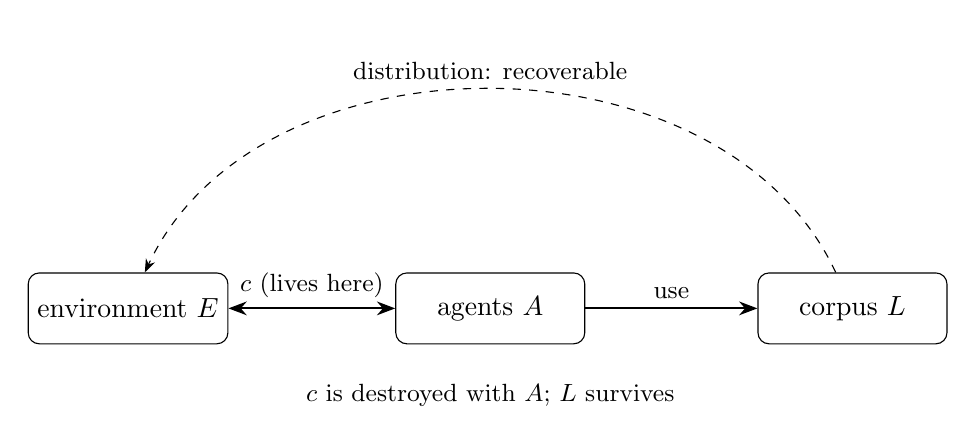
\begin{tikzpicture}[>=Stealth,node distance=1.2cm]
\node[draw,rounded corners,minimum width=2.4cm,minimum height=0.9cm] (E) at (0,0) {environment $E$};
\node[draw,rounded corners,minimum width=2.4cm,minimum height=0.9cm] (A) at (4.6,0) {agents $A$};
\node[draw,rounded corners,minimum width=2.4cm,minimum height=0.9cm] (L) at (9.2,0) {corpus $L$};
\draw[<->,thick] (E) -- node[above,font=\small] {$c$ (lives here)} (A);
\draw[->,thick] (A) -- node[above,font=\small] {use} (L);
\draw[->,dashed] (L) to[out=115,in=65] node[above,font=\small] {distribution: recoverable} (E);
\node[font=\small] at (4.6,-1.1) {$c$ is destroyed with $A$; $L$ survives};
\end{tikzpicture}
\caption{The correspondence $c$ is a relation between environment and agents. The corpus
is downstream. Recovering the distribution over $L$ does not recover $c$, and the dashed
arrow is not a reconstruction of $c$ but a statistic of its traces.}
\label{fig:locus}
\end{figure}

\section{Why the mortal scientist does not face this problem}
\label{sec:scientist}

The mortal-scientist framework models a learner as a cost-accounted computation in the
reflective higher-order calculus, with hypotheses drawn from a namespace logic whose
formulae denote bisimulation equivalence classes.\footnote{The calculus is written
\rc{}, never $\rho$. The name is an acronym for \emph{reflective higher order}; that it
reads as the Greek letter following $\pi$ is a pun on the rho calculus following the
$\pi$-calculus, not an assertion that the letter is the name.} It is worth being clear
about why that
framework does not encounter the bootstrap problem, because the reason is instructive and
is not that the problem was solved.

Computations are ontologically isolated, so the environment of a computation is other
computations. Both sides of the cut are therefore objects of the same calculus. The
hypothesis language is a logic for that calculus, and its formulae denote equivalence
classes of exactly the things on the far side of the cut. The correspondence between
symbol and referent is consequently \emph{analytic}: there is no gap to bridge because
the ontology and the hypothesis language are two presentations of one object. The
scientist's grounding is perfect in the limit for the same reason that a map of a map is
accurate---the territory was chosen to be of the same kind as the map.

\begin{observation}[The sidestep]
\label{obs:sidestep}
The mortal scientist's grounding is guaranteed by the coincidence of the model of
computation with the model of the environment. Every result of that framework which
relies on both sides of the cut being \rc{}-processes requires re-derivation when the far
side is not.
\end{observation}

\noindent This is not a criticism of the framework, which was built for a different
purpose and does that job. It is a statement of scope. The moment we ask for a mind that
acts in the world humans act in, the far side of the cut stops being a \rc{}-process and
Observation~\ref{obs:sidestep} takes effect. Everything in \S\S\ref{sec:goodman}--\ref{sec:rho}
is an attempt to say what would have to be added.

\section{Goodman's framework, provisionally adopted}
\label{sec:goodman}

\subsection{Why this framework}

The bootstrap problem asks us to construct a symbol system. It is therefore prior to ask
what one is. The literature reviewed above is remarkably thin on this: symbol grounding
work generally treats ``symbol'' as understood and asks how to attach it to sensors;
representation learning treats discreteness as an architectural choice; emergent
communication treats a symbol as whatever the channel carries. None of these gives a
criterion by which a proposed system could be judged inadequate.

Goodman's \emph{Languages of Art} does \cite{goodman1968}. It offers a set of conditions
distinguishing notational systems from other symbol systems, developed for the score /
performance relation in music and dance and generalised from there. We adopt it
provisionally---provisionally because it has known failure modes, discussed in
\S\ref{sec:failures}, and because adopting it is a bet that its conditions are the right
ones rather than merely the first available ones.

The one prior attempt to put Goodman's theory to computational work is Goel's, which
derives from notationality a class of \emph{physical notational systems} and argues that
these are exactly the dynamical systems capable of realising computational information
processing \cite{goel1991}. That work predates the current setting and has not been
revisited for learned representations. It is, so far as we can determine, the whole of
the prior art.

\subsection{The conditions}

Goodman's apparatus distinguishes \emph{marks} (physical inscriptions or utterances),
\emph{characters} (classes of marks that count as the same), and \emph{compliants} (the
things a character applies to, its \emph{compliance class}). A score is a character; a
performance is a compliant.

A \emph{notational scheme} satisfies two syntactic conditions:

\begin{condition}[Syntactic disjointness]
\label{cond:sd}
No mark belongs to more than one character.
\end{condition}

\begin{condition}[Syntactic finite differentiation]
\label{cond:sfd}
For any two characters $K \neq K'$ and any mark $m$ not belonging to both, it is
theoretically possible to determine that $m$ does not belong to $K$, or that it does not
belong to $K'$.
\end{condition}

\noindent A \emph{notational system} is a scheme satisfying three further semantic
conditions:

\begin{condition}[Unambiguity]
\label{cond:ua}
Each character has a single compliance class: not different compliants at different times
or in different contexts.
\end{condition}

\begin{condition}[Semantic disjointness]
\label{cond:semd}
No two characters share a compliant.
\end{condition}

\begin{condition}[Semantic finite differentiation]
\label{cond:semfd}
The analogue of Condition~\ref{cond:sfd} on the compliance side.
\end{condition}

\noindent The two finite-differentiation conditions are what exclude \emph{dense} systems.
A system whose characters are ordered so that between any two there is a third fails
Condition~\ref{cond:sfd}, and this is Goodman's account of the difference between a score
and a sketch, or between digital and analogue.

\subsection{The roundtrip is derived, not primitive}

It is natural---and was our own first reading---to take the criterion of adequacy to be
losslessness of the roundtrip: from score to performance and back by transcription, and
from performance to score and back, without loss of identity. That is indeed the property
Goodman is after, and it is the property that matters for our purposes. But it is a
consequence of Conditions~\ref{cond:sd}--\ref{cond:semfd}, not an additional stipulation,
and the distinction is load-bearing. The roundtrip tells you when you have succeeded. The
five conditions tell you what to check, and they decompose the requirement into parts that
turn out to have very different relationships to the machinery we have.

\begin{remark}[What the framework does and does not do]
\label{rem:invariance}
Goodman's conditions are conditions on a symbol \emph{system}: a scheme together with a
compliance relation. They presuppose the compliance relation as given and adjudicate
whether it is notational. They therefore cannot \emph{select} a compliance relation, and
they are invariant under relabelling: if $\Sigma$ is a notational system and $\phi$ is a
bijection on characters, $\phi(\Sigma)$ is a notational system with the same compliance
classes differently named. Consequently Goodman's framework says what a solution to the
bootstrap problem would look like, and cannot by itself produce one.
\end{remark}

\noindent Remark~\ref{rem:invariance} is the reason this note describes the adoption of
Goodman as ``half the battle'' rather than as progress on the bootstrap problem proper. It
returns with force in \S\ref{sec:social}.

\subsection{Failure modes and provisional repairs}
\label{sec:failures}

\paragraph{The wrong-note paradox.} Goodman's compliance relation is exact: a performance
containing a single wrong note is not a performance of the work. Since performances
without wrong notes are essentially never found, the theory as stated has no instances in
musical practice. This is the standard objection and it is a real one.

We record the shape of the repair now and return to it in \S\ref{sec:budget}: exactness
should be relativised to a resource bound. Two performances are the same performance if no
affordable observation separates them. This is not an evasion, because in a cost-accounted
setting ``affordable'' is a defined quantity rather than a hand-wave, and it converts an
absolute condition into a family of conditions indexed by budget.

\paragraph{Density is a property of the world, not only of the notation.} Finite
differentiation can fail because the notation is badly designed, or because the phenomenon
being notated is dense and no notation of it can succeed. Goodman does not clearly
separate these, and for the bootstrap problem the separation is essential: we need to know
whether a failure to notate is a failure of the agent or a fact about the environment. See
Question~\ref{q:density}.

\paragraph{The ontological commitments are separable.} Goodman's theory of notation comes
attached to strong claims about the identity of works of art. Recent work in aesthetics
argues that the notational apparatus survives being detached from those commitments and
reinterpreted epistemically \cite{estetika2026}. We take that detachment for granted here.

\section{Fit with a bisimulation-based approach}
\label{sec:bisim}

\subsection{The two bisimulations}

The natural translation of the roundtrip requirement into process-calculus vocabulary is a
pair of bisimulations. Write $\mathcal{S}$ for the space of scores, $\mathcal{P}$ for the
space of performances, $\llbracket-\rrbracket : \mathcal{S} \to \mathcal{P}(\mathcal{P})$
for the compliance map taking a score to its compliance class, and
$\tau : \mathcal{P} \to \mathcal{S}$ for transcription. The requirement is that

\begin{align}
p \bisim_{\mathcal{P}} p' &\iff \tau(p) \bisim_{\mathcal{S}} \tau(p') \label{eq:rt1}\\
s \bisim_{\mathcal{S}} s' &\iff \llbracket s \rrbracket = \llbracket s' \rrbracket \label{eq:rt2}
\end{align}

\noindent with $\bisim_{\mathcal{P}}$ and $\bisim_{\mathcal{S}}$ the respective
behavioural equivalences. Read one way this says the two kernels agree; read another, that
$\tau$ and $\llbracket-\rrbracket$ are mutually inverse on the quotients.

\subsection{What bisimulation supplies}

Conditions \ref{cond:sd}, \ref{cond:ua} and \ref{cond:semd} are quotient conditions and
fall out of \eqref{eq:rt1}--\eqref{eq:rt2} directly. Syntactic disjointness says the
character map is a function on marks, which is what it means for $\bisim_{\mathcal{S}}$ to
be an equivalence. Unambiguity says the compliance class of a character does not vary,
which is a statement that $\llbracket-\rrbracket$ is well defined on
$\bisim_{\mathcal{S}}$-classes. Semantic disjointness says compliance classes partition,
which is \eqref{eq:rt2} read as injectivity on the quotient.

This is a good fit, and it is why the translation is worth making at all. Bisimulation is
the mathematically mature version of ``same behaviour'', it comes with coinductive proof
methods, and in the reflective setting it is the equivalence the logic already denotes.

\subsection{Where Goodman adds}
\label{sec:adds}

Conditions \ref{cond:sfd} and \ref{cond:semfd} are \emph{not} quotient conditions and
bisimulation does not supply them.

\begin{observation}[Separation is not quotient]
\label{obs:sep}
Finite differentiation is a separation condition: it requires not merely that distinct
characters be distinct, but that their distinctness be \emph{effectively determinable}
from a mark. A bisimulation quotient can be perfectly well defined over a dense space,
in which case every pair of distinct classes is distinguishable in the limit and no pair
is distinguishable by any finite observation. Such a system satisfies
\eqref{eq:rt1}--\eqref{eq:rt2} and fails Condition~\ref{cond:sfd}.
\end{observation}

\noindent This is the precise content of ``Goodman is compatible with the bisimulation
approach but adds more conditions''. What he adds is an effectivity requirement that
process equivalence, being defined by a greatest fixed point, is systematically silent
about.

The point is not academic. It is exactly where the neural implementations fail.

\subsection{Two empirical instances of the gap}
\label{sec:instances}

\paragraph{LatPlan and the symbol stability problem.} LatPlan learns propositional and
action symbols from unlabelled image pairs and plans in the resulting latent space
\cite{asai2018}. Asai and Kajino subsequently identified what they named the
\emph{symbol stability problem}: the propositions produced by the state autoencoder behave
stochastically, so the same input does not reliably produce the same proposition
\cite{asai2019}. In Goodman's vocabulary this is a failure of
Condition~\ref{cond:sfd}---one mark, no effective determination of which character it
belongs to---and it was discovered empirically, without the vocabulary, as an obstacle to
making a learned symbol system behave like a symbol system.

\paragraph{Vector quantisation as a fix for one condition only.} The VQ-VAE bottleneck
assigns continuous latents to a codebook by nearest neighbour \cite{oord2017}. This
imposes syntactic disjointness and a separation margin by construction: it is, read
through Goodman, an engineering solution to Conditions~\ref{cond:sd} and \ref{cond:sfd}
and to nothing else. It says nothing about the compliance side, which is why quantisation
alone does not produce symbols that mean anything. The subsequent literature's efforts to
make the codes ``semantic'' by additional training objectives are attempts to buy
Conditions~\ref{cond:ua}--\ref{cond:semfd} that do not know they are doing so.

\subsection{Why bisimulation metrics are the wrong repair}

The reinforcement-learning literature has independently encountered the rigidity of exact
bisimulation and responded with quantitative relaxations: bisimulation metrics
\cite{ferns2004} and their scalable descendants \cite{gelada2019,zhang2021,castro2021}.
These are the correct response to the wrong-note paradox in that setting, and they are the
wrong response here.

\begin{observation}[The metric smooths what notation needs separated]
\label{obs:metric}
A bisimulation metric replaces the equivalence with a distance and the quotient with a
geometry. It thereby dissolves precisely the discreteness that
Conditions~\ref{cond:sfd} and \ref{cond:semfd} require. A representation shaped by a
bisimulation metric is, in Goodman's classification, closer to a sketch than to a score.
\end{observation}

\noindent The tension is genuine and not merely terminological. One cannot have a symbol
system and a smooth behavioural geometry at the same level of description. What one can
have is a discrete system whose \emph{admissible discriminations} are set by a resource
bound, which is the next subsection.

\subsection{Budget-relative separation}
\label{sec:budget}

The mortal-scientist framework already prices observation: assays cost, refutation is
budget-relative, and a verdict may be $\bot$ because the budget ran out rather than
because the world was silent. This supplies exactly the ingredient
Observation~\ref{obs:sep} says is missing.

\begin{conjecture}[Finite differentiation as a theorem]
\label{conj:fd}
In a cost-accounted setting with budget $\sigma$, define $x \bisim^{\sigma} y$ to hold
when no assay affordable at $\sigma$ separates $x$ from $y$. Then the quotient by
$\bisim^{\sigma}$ satisfies Conditions~\ref{cond:sfd} and \ref{cond:semfd} with the
budget as the separation constant, and the resulting family
$\{\Qs\}_{\sigma}$ is a filtered diagram of notational schemes refining as
$\sigma$ grows.
\end{conjecture}

\noindent We state this as a conjecture rather than a proposition because two things are
unverified. First, that $\bisim^{\sigma}$ is transitive: affordability is not obviously
composable, and a chain of pairwise-indistinguishable states may have distinguishable
endpoints, which is the standard failure of ``indistinguishable by a bounded observer''
relations. Second, that the cost-accounting monad interacts correctly with the extension
of \S\ref{sec:rho}; see Question~\ref{q:monad}. If the first fails, the repair is to take
the transitive closure and accept a coarser scheme, at the price of the separation
constant no longer being $\sigma$.

Should Conjecture~\ref{conj:fd} hold, it has an appealing reading: a poorer agent has a
coarser notation, notational adequacy is a purchasable property, and the wrong-note
paradox is resolved by making exactness relative to what can be afforded rather than by
abandoning it.

\section{\rc{} and builtin processes}
\label{sec:rho}

\subsection{Reflection is score construction, not performance}
\label{sec:scoreconstruction}

The reflective higher-order calculus takes names to be quoted processes
\cite{meredith2005}. For a process $P$, $\quo{P}$ is a name; for a name $x$, $*x$ is a
process; and $*\quo{P} = P$, $\quo{*x} = x$. Quotation and dereference are mutually
inverse.

It is tempting---and we made this mistake before correcting it---to read this immediately
as the score / performance relation with Goodman's roundtrip holding by construction. It is
not, and seeing why is what makes the rest of this section follow rather than intrude.

In pure \rc{}, both sides of $\quo{-}$ and $*$ are syntax. $P$ is a term; $\quo{P}$ is a
term-code; $*\quo{P}$ is the same term again. Nothing here is a performance. What the
operators do is build scores out of scores: quotation lets a score be embedded in another
score as an atom, and dereference recovers it. The construction is \emph{recursive score
construction}, and its losslessness is the statement that the recursion is faithful---that
no information is lost by descending a level and climbing back. That is a genuine and
useful property, but it is a property internal to the notation. A notational system all of
whose compliants are further inscriptions is exactly the case Goodman analyses under the
heading of scripts that denote other scripts, and it is not yet a system that says anything
about a world.

\begin{observation}[Two readings of $\quo{-}$ and $*$]
\label{obs:tworeadings}
In $\rc = \RHO[\varnothing]$, $\quo{-}$ and $*$ are score-to-score: they witness the
faithfulness of a recursion inside the notation, and there is no performance in the picture.
The compliance relation is trivial in the sense that every character complies with syntax.
\end{observation}

\subsection{Builtins turn the recursion into a correspondence}
\label{sec:turn}

Now adjoin a builtin process $b$ drawn from the host world. The syntax of quotation does
not change: $\quo{b}$ is formed exactly as $\quo{P}$ is. But its \emph{semantics} changes
completely, because $b$ is not a term of the calculus. It is a behaviour in the world the
computation is embedded in.

At that point, and only at that point, $\quo{b}$ is a score and $b$ is a performance in
Goodman's sense. $\quo{b}$ is a static, inspectable, transmissible mark that can be handled
by \rc{}'s own machinery---sent on channels, pattern-matched, quantified over in the
namespace logic---while the thing it codes is an event elsewhere, running under laws the
calculus does not supply. Dereference $*\quo{b}$ is then not a syntactic identity but a
performance instruction: it says, produce in the host world something indistinguishable
from $b$.

\begin{observation}[Where the correspondence enters]
\label{obs:enters}
Adjoining builtins does not add a new operator. It re-types the existing one. The same
$\quo{-}$ that was recursive score construction over \rc{}-terms becomes, on the builtin
sort, a score / performance correspondence; and the same $*$ that was syntactic recovery
becomes performance. Goodman's roundtrip requirement therefore attaches to \rc{} at exactly
the point where the calculus is extended by the world, and nowhere else.
\end{observation}

\noindent This is why the extension is the interesting object and the pure calculus is not.
In $\RHO[\varnothing]$ there is nothing to ground and the roundtrip is a tautology. In
$\RHO[\Bee]$ the roundtrip is a claim about the relation between a term language and a
world, which is the kind of claim the bootstrap problem is about. Everything the rest of
this section does is take that observation seriously and see how far it can be pushed---and
\S\ref{sec:notasolution} argues that the answer is: not far enough.

\subsection{Two ways to adjoin the world}

There are two ways to perform the extension, and Observation~\ref{obs:enters} explains why
only one of them does the job.

\paragraph{Builtin names.} Adjoin name constants beyond $\quo{0}$, understood as channels
to the host world. This gives an interface but no theory of what is on the other end: the
calculus can send and receive, and has nothing to say about the behaviour it is
interacting with. It is the applied-$\pi$ move \cite{abadi2001}, where a term algebra of
data is adjoined and the added material is inert with respect to the operational
semantics. Crucially, it does \emph{not} re-type $\quo{-}$: an adjoined name is a name, not
the quotation of anything, so there is no performance for it to be the score of, and
Observation~\ref{obs:tworeadings} still applies. The roundtrip stays inside the notation.

\paragraph{Builtin processes.} Adjoin processes $b$ drawn from the host world. Then
$\quo{b}$ is a \emph{symbol for} $b$, and $*\quo{b}$ is a process in the host world
indistinguishable from $b$. This is the version that does the work, for the reason just
given: it is the only one of the two under which quotation acquires a compliance class
outside the syntax.

\begin{remark}[This is not psi-calculi]
The psi-calculi framework parameterises $\pi$-like calculi by nominal datatypes for terms,
conditions and assertions, together with a channel-equivalence relation, a composition, a
unit and an entailment relation, and subsumes applied $\pi$, spi, fusion and concurrent
constraint $\pi$ as instances \cite{bengtson2011}. The adjoined material there is
\emph{data}: inert under the operational semantics, transmitted but not run. Adjoining
builtin \emph{processes} is a different move, because the adjoined objects have their own
dynamics and the calculus ceases to be closed---part of the reduction relation is
delegated to the host. Readers who know psi-calculi will otherwise assume this is an
instance of it.
\end{remark}

\subsection{The calculus-making functor}

The natural way to organise this is to stop thinking of \rc{} as a calculus and think of
it as a functor from behaviours to calculi:
\[
\RHO[\Bee] ::= 0 \mid \Bee \mid \mathtt{for}(y \Leftarrow x)P \mid x!(Q) \mid P \mid Q
\mid *x, \qquad x, y ::= \quo{P}
\]
with the usual equations and rewrites, and with $\Bee$'s behaviour specified in a source
category $\Cat$ and imported into a version of the parallel-composition rule. The pure
calculus is then the fibre over the empty behaviour, $\rc = \RHO[\varnothing]$, and
everything previously done with \rc{} has been done in that fibre.

\subsection{What the functorial reading suggests}
\label{sec:suggests}

Four things, each of which is a suggestion rather than a theorem.

\paragraph{(i) The import into $\mid$ has a known shape.} ``Behaviour specified in the
source category, imported into the par rule'' is the shape of a distributive law of syntax
over behaviour. Turi and Plotkin's bialgebraic semantics takes operational rules given as a
natural transformation $\lambda : SF \Rightarrow FS^{\dagger}$, with $S$ a syntax functor,
$F$ a behaviour functor and $S^{\dagger}$ the free monad on $S$, and yields an operational
model together with a canonical, internally fully abstract denotational model
\cite{turi1997}. The relevant corollary is that for any such law, behavioural equivalence
in the final coalgebra is a congruence on the operational model. If the import can be put
in that form, bisimulation-as-congruence over $\RHO[\Bee]$ comes free rather than being
re-proved per $\Bee$. If it cannot, congruence fails and every compositional result of the
existing notes stops transferring across the cut. This is checkable and unchecked.

\paragraph{(ii) Functoriality is the roundtrip.} Take the morphisms of $\Cat$ to be
behaviour-preserving maps. There is then a unit $\eta_{\Bee} : \Bee \to \RHO[\Bee]$
including builtins as processes, and:
\begin{itemize}[leftmargin=1.6em]
\item $\eta$ faithful says distinct builtin behaviours receive distinct symbols, which is
performance $\to$ score $\to$ performance losslessness;
\item $\eta$ full says every \rc{}-level distinction over builtins is realised by a
builtin distinction, which is score $\to$ performance $\to$ score losslessness, and which
forbids the calculus from minting symbols the world cannot cash.
\end{itemize}
So Goodman's criterion of adequacy becomes the statement that $\eta_{\Bee}$ is full and
faithful with respect to behavioural equivalence. That is a property one could try to
prove, which is more than the criterion was before.

\paragraph{(iii) Unambiguity forces behaviours, not states.} If the objects of $\Bee$ are
states with dynamics, then $\quo{b}$ codes a moving target: the same mark has different
compliants at different times, which is exactly the failure of Condition~\ref{cond:ua}.
The repair is forced: the objects of $\Bee$ must be \emph{behaviours}---a subobject of the
final $F$-coalgebra---so that quoting a builtin quotes its entire future rather than a
snapshot. Then $*\quo{b} \bisim b$ holds definitionally, and unambiguity holds because
behaviours do not change over time even though states do. A consequence worth stating: one
cannot take $\Bee$ to be the physical furniture of the world. $\Bee$ must be the world
already quotiented by an observational equivalence, which is where
Conjecture~\ref{conj:fd} would enter, with $\Bee = \Qs(W)$.

\paragraph{(iv) The source category is constrained.} Name matching in
$\mathtt{for}(y \Leftarrow x)P \mid x!(Q)$ requires deciding name equality, and names now
include $\quo{b}$. So structural congruence on $\RHO[\Bee]$ is decidable only if equality
on $\Bee$'s objects is at least budget-decidable. This is a restriction on which worlds
can serve as source, and it is the formal descendant of the observation that builtin names
are the base case of the well-founded coding by which quotation manufactures fresh names.

\begin{figure}[t]
\centering
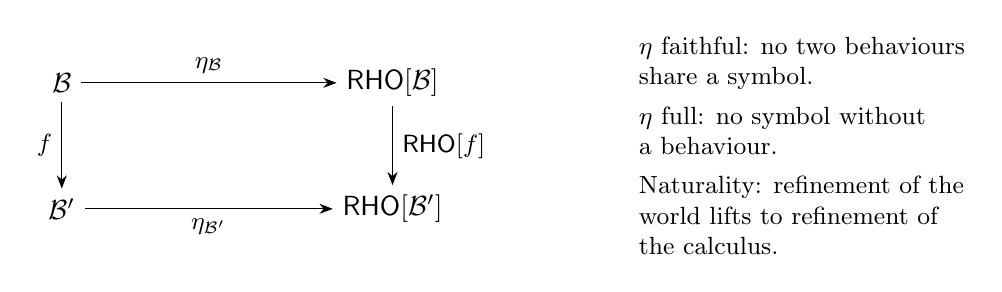
\begin{tikzpicture}[>=Stealth,node distance=2.2cm]
\node (B) at (0,1.6) {$\Bee$};
\node (RB) at (4.2,1.6) {$\RHO[\Bee]$};
\node (B2) at (0,0) {$\Bee'$};
\node (RB2) at (4.2,0) {$\RHO[\Bee']$};
\draw[->] (B) -- node[above,font=\small] {$\eta_{\Bee}$} (RB);
\draw[->] (B2) -- node[below,font=\small] {$\eta_{\Bee'}$} (RB2);
\draw[->] (B) -- node[left,font=\small] {$f$} (B2);
\draw[->] (RB) -- node[right,font=\small] {$\RHO[f]$} (RB2);
\node[font=\small,align=left] at (9.4,0.8)
 {$\eta$ faithful: no two behaviours\\ share a symbol.\\[0.35em]
  $\eta$ full: no symbol without\\ a behaviour.\\[0.35em]
  Naturality: refinement of the\\ world lifts to refinement of\\ the calculus.};
\end{tikzpicture}
\caption{The functorial reading. Goodman's two-way losslessness becomes fullness and
faithfulness of the unit; extensibility of the builtin set becomes naturality in $\Bee$.}
\label{fig:functor}
\end{figure}

\subsection{Why this is an analogy and not a solution}
\label{sec:notasolution}

We now argue against the construction just presented, because the argument is short and
decisive and it is better made here than by a reader.

\begin{enumerate}[label=\textbf{(\alph*)},leftmargin=2.4em]

\item \textbf{It consumes what it was meant to produce.} $\RHO[-]$ takes $\Bee$ as an
argument. The bootstrap problem is the problem of \emph{finding} $\Bee$: of individuating
the world into behaviours worth having symbols for. The functor presupposes a solved
instance of the problem it was introduced to address, and everything it then does is
bookkeeping over that solution. This is the decisive objection and the rest are
supporting.

\item \textbf{Functoriality entails relabelling invariance.} $\RHO[\Bee] \cong
\RHO[\Bee']$ whenever $\Bee \cong \Bee'$. So the construction cannot fix reference; it
transports whatever reference $\Bee$ came with. Note that this is not an imported
objection but a theorem of the construction, and it is the formal version of
Remark~\ref{rem:invariance}.

\item \textbf{Losslessness is stipulated where it is interesting.} $*\quo{b} \bisim b$
holds by construction because we defined $\quo{-}$ on $\Bee$ to be exact. In the world,
sensor-to-symbol transduction is lossy, noisy and partial, and the interesting question is
what to do when the roundtrip \emph{fails}. The construction has nothing to say about
approximate compliance, which is where all the empirical difficulty lives.

\item \textbf{The par rule import is unverified.} \S\ref{sec:suggests}(i) is conditional.
Until the import is exhibited as a distributive law of the required shape, congruence of
bisimulation over $\RHO[\Bee]$ is an assumption, and with it every compositional result
that would be transported.

\item \textbf{Two interaction disciplines complicate the logic.} \rc{} communication is
name-mediated. If builtins react in the source category by something that is not a name
rendezvous, $\RHO[\Bee]$'s parallel composition hosts two kinds of redex, and the
namespace logic's modalities---which quantify over redex positions---require a sort
distinction. The ladders computed in the existing notes would need recomputation, and it
is not known whether their qualitative shape survives.

\item \textbf{Nothing here proposes candidates.} Even granting all of the above, the
construction is a specification language for grounded symbol systems, not a procedure for
acquiring one. It says what the answer must look like. It does not search.

\end{enumerate}

\noindent The honest summary is that the functorial reading is a good way to \emph{state}
several of Goodman's conditions in a form where they might be proved, and no way at all to
satisfy them.

\section{Reference cannot be fixed from inside}
\label{sec:social}

One consequence of \S\ref{sec:notasolution}(b) deserves separate statement, because it
changes the shape of the project rather than merely qualifying it.

Suppose an agent solves the bootstrap problem in the sense stated: it constructs a symbol
system, its own, notationally adequate, with correspondence to its environment
instantiated in itself. Nothing in that achievement makes the system correspond to
\emph{our} symbols. By Remark~\ref{rem:invariance} and \S\ref{sec:notasolution}(b), the
system is determined up to isomorphism and no further. A grounded but idiosyncratic symbol
system is Rongorongo viewed from the other side: perfectly meaningful to its users,
opaque to everyone else, and opaque for exactly the reason given in
Observation~\ref{obs:locus}.

\begin{observation}[The social term is forced]
\label{obs:social}
For the target ``a mind that acts in the world humans act in'', grounding is a property of
a composite of at least two agents with shared action, not of any single agent. Any
framework that is invariant under relabelling of a single agent's symbols cannot deliver
the target, and $\RHO[-]$ is such a framework by construction.
\end{observation}

\noindent This is the point at which the emergent-communication literature stops being
adjacent and starts being load-bearing. It is also where the argument of this section
meets the existence proofs of \S\ref{sec:soluble} coming the other way: relabelling-%
invariance says a single agent \emph{cannot} fix reference, and the only two known
solutions to the bootstrap problem were both achieved by populations and by neither
lineage's individuals. A structural argument and an empirical one, with no premises in
common, reaching the same requirement. Steels's language-game experiments demonstrate
shared vocabulary arising between embodied agents through repeated situated interaction
\cite{steels2015}, and Taniguchi's collective predictive coding hypothesis reconstructs
the phenomenon as decentralised Bayesian inference over latent variables that are common
nodes connecting many agents, achievable without connecting brains
\cite{taniguchi2024}. Neither solves the bootstrap problem---both assume pre-segmented
perceptual channels, which is objection \S\ref{sec:notasolution}(a) again---but both
supply the ingredient a single-agent account structurally cannot.

For the present programme the practical consequence is that \emph{Composing Learners} is
not an extension of the mortal-scientist framework but a prerequisite for the grounding
question. A learner as a distribution over a population, composed by parallel composition
with typed namespace overlap, is the right shape of object to carry a correspondence that
no member of the population carries alone.

\section{Where a transformer belongs}
\label{sec:transformer}

The framing above assigns transformers a job, and it is not the job they are usually given
in discussions of grounding.

In the construction of \S\ref{sec:rho} the transducer is $\quo{-}$ and $*$ extended to
builtins. That map is exact and lossless by construction; a network cannot improve on it
and is not needed for it. What is needed, and what nothing in the calculus supplies, is a
\emph{proposal mechanism}: given a stream of host-world observation, propose candidate
builtin behaviours. This is objection \S\ref{sec:notasolution}(a) turned into a task.

Two features make it a well-posed learning problem, which is more than can be said for
``learn symbols from sensors''.

\paragraph{The success criterion is coverage, not reward.} $\Bee$ is a \emph{presentation}:
a generating set such that the observable world lies in the image of $\RHO[\Bee]$. This is
a generators-and-relations problem with a definite answer, and minimality of $\Bee$ is a
statistical-complexity analogue rather than a hyperparameter.

\paragraph{There is a principled candidate.} Causal states are already the coarsest
coarse-graining of pasts retaining full predictive power \cite{shalizi2001}, and by
\S\ref{sec:recovers} a next-token-trained transformer represents belief states over them
\cite{shai2024}. That makes causal states the natural first candidate for which
distinctions deserve builtin names. The correspondence extends further than convenience:
Crutchfield's taxonomy of $\epsilon$-machines runs from finite-state through countable to
uncountable and fractal, and that taxonomy \emph{is} a density hierarchy---so
Condition~\ref{cond:sfd} is the condition separating its bottom rung from the rest, and
``is this world notationally accessible to this agent at this budget'' becomes ``is the
budget-quotiented $\epsilon$-machine of the host process finite''.

The second job for a network is amortised bisimulation checking. Assays are priced in the
existing framework, checking behavioural equivalence is expensive, and an approximate
checker with calibrated error is a legitimate purchase if its errors can be priced. This
is more speculative and we do not pursue it here.

\section{Open questions}
\label{sec:open}

\paragraph{On the notational apparatus.}

\begin{question}[Transitivity of budget-relative indistinguishability]
\label{q:trans}
Is $\bisim^{\sigma}$ of Conjecture~\ref{conj:fd} transitive? If not, what is the cost of
taking transitive closure, and does the resulting scheme still separate at a rate related
to $\sigma$?
\end{question}

\begin{question}[Density: agent or world?]
\label{q:density}
Given a failure of Condition~\ref{cond:sfd}, is there a criterion separating ``this agent
cannot notate this world'' from ``this world admits no notation''? A candidate: the
former is a statement about $\Qs$ for the agent's $\sigma$, the latter about
$\lim_{\sigma \to \infty} \Qs$.
\end{question}

\begin{question}[Notationality of learned codebooks]
Goodman's five conditions are checkable properties of an encoder / decoder pair. What do
VQ-VAE codebooks, BPE tokenisers and LatPlan's state autoencoder score on them? ``How
notational is this tokeniser'' appears to be a measurable quantity and, so far as we can
determine, has never been measured.
\end{question}

\paragraph{On the functor.}

\begin{question}[Is the import a distributive law?]
\label{q:gsos}
Can the import of $\Bee$'s behaviour into parallel composition be exhibited as
$\lambda : \RHO \circ F \Rightarrow F \circ \RHO^{\dagger}$? If so, congruence is free by
\cite{turi1997}. If not, what weaker condition holds, and does the lax version suffice?
\end{question}

\begin{question}[Is $\RHO$ a monad?]
\label{q:monad2}
Does $\RHO[\RHO[\Bee]] \to \RHO[\Bee]$ flatten? If so its algebras are the worlds closed
under \rc{}-computation, which would be a sharp notion of ``a world that can host''. Note
that abstract GSOS wants the syntax as a monad or its free monad, so this question and
Question~\ref{q:gsos} are coupled.
\end{question}

\begin{question}[Does $\RHO$ preserve the cost-accounting monad?]
\label{q:monad}
The existing notes work inside plain \rc{} and appeal to a WLOG on syntax that is valid
there. If cost accounting is a monad $T$, do $\RHO[-]$ and $T$ commute? If they do not,
the foraging inequality, the pricing schedule and the monotonicity of cost in distance do
not transport to $\RHO[\Bee]$, and with them Conjecture~\ref{conj:fd} loses its setting.
\end{question}

\begin{question}[Full and faithful $\eta$]
For which source categories $\Cat$ and which subobjects $\Bee$ of the final coalgebra is
$\eta_{\Bee}$ full and faithful with respect to weak bisimulation? Failure of fullness
would be the calculus minting uncashable symbols, which is a diagnosable pathology and
possibly a measurable one.
\end{question}

\begin{question}[Sorting the logic]
If $\RHO[\Bee]$ hosts two kinds of redex, what is the corresponding refinement of the
namespace logic's modalities, and does the qualitative shape of the ladders computed in
\emph{Learning to Play} and \emph{Composing Learners} survive it?
\end{question}

\paragraph{On the bootstrap proper.}

\begin{question}[Proposing $\Bee$]
Given host-world observation, what proposes candidate builtin behaviours, and against what
loss? \S\ref{sec:transformer} argues the criterion is coverage of the observable world by
$\RHO[\Bee]$. Making that a differentiable or otherwise optimisable objective is open.
\end{question}

\begin{question}[Extensibility]
Acquiring a new distinction should be a morphism $\Bee \to \Bee'$ in $\Cat$ that $\RHO$
transports. What is the well-founded discipline under which an agent may extend its own
builtin set---presumably by quotation over existing builtins, which is the algebraic form
of generate-and-test feature construction in the sense of \cite{pierce1997}?
\end{question}

\begin{question}[The minimal social configuration]
Observation~\ref{obs:social} says grounding is a property of a composite. What is the
smallest composite that suffices? Two agents with shared action, or does the argument
require a population? Does the typed-overlap apparatus of \emph{Composing Learners}
already contain the answer?
\end{question}

\begin{question}[Approximate compliance]
\S\ref{sec:notasolution}(c) observes that the interesting case is roundtrip failure. Is
there a notion of \emph{graded} compliance that degrades Goodman's conditions gracefully
without collapsing into the metric of Observation~\ref{obs:metric}?
\end{question}

\section{What is claimed and what is not}
\label{sec:claims}

\paragraph{Claimed.} That the correspondence between a language and a world is a fact
about the language's users and is not contained in the corpus
(Observation~\ref{obs:locus}); that the record of decipherment and of cetacean
bioacoustics is evidence for this rather than merely consistent with it, and that the two
successful routes both acquire the correspondence from agents who already have it
(Observation~\ref{obs:transport}); that next-token
prediction recovers the structure of the token-generating process, which for a corpus is
the linguistic community and not the environment (Observation~\ref{obs:generator}); that
the problem has at least two independent solutions in nature, so that solubility is not in
question and impossibility arguments are unsound (Observation~\ref{obs:soluble}); that
the mortal-scientist framework's grounding is analytic and therefore does not address this
(Observation~\ref{obs:sidestep}); that Goodman's conditions decompose into quotient
conditions that bisimulation supplies and separation conditions that it does not
(Observation~\ref{obs:sep}); that bisimulation metrics are the wrong repair for the latter
(Observation~\ref{obs:metric}); that quotation and dereference in the pure calculus are
score-internal recursion and acquire a compliance class outside the syntax only when
builtin processes are adjoined (Observations~\ref{obs:tworeadings} and \ref{obs:enters});
and that no relabelling-invariant single-agent framework
can deliver correspondence to \emph{human} symbols (Observation~\ref{obs:social}).

\paragraph{Conjectured.} That cost accounting supplies finite differentiation with the
budget as separation constant (Conjecture~\ref{conj:fd}).

\paragraph{Offered as analogy only.} The entire content of \S\ref{sec:rho}. The functorial
reading organises the conditions attractively and suggests four checkable statements. It
does not bootstrap anything, for the reasons given in \S\ref{sec:notasolution}, and the
first of those reasons is not a technicality.

\paragraph{Not claimed.} That Goodman's conditions are the right ones---they are adopted
provisionally, and the density and wrong-note objections are live. That transformers
cannot in principle transduce---only that next-token prediction over an already-grounded
corpus is not transduction, and that the two are routinely conflated. That the bootstrap
problem is soluble \emph{by construction}: nature's two solutions were achieved by
populations, under selection, over long timescales, with interfaces that co-evolved with
the symbol systems they support, and this note has no argument that any of those
conditions can be dispensed with.

\begin{thebibliography}{99}

\bibitem{abadi2001} M. Abadi and C. Fournet. Mobile values, new names, and secure
communication. \emph{POPL}, 2001.

\bibitem{asai2018} M. Asai and A. Fukunaga. Classical planning in deep latent space:
bridging the subsymbolic-symbolic boundary. \emph{AAAI}, 2018.

\bibitem{asai2019} M. Asai and H. Kajino. Towards stable symbol grounding with
zero-suppressed state autoencoder. \emph{ICAPS}, 2019.

\bibitem{benderkoller2020} E. M. Bender and A. Koller. Climbing towards NLU: on meaning,
form, and understanding in the age of data. \emph{ACL}, 2020.

\bibitem{begus2026} G. Beguš, M. Dąbkowski, R. L. Sprouse, D. F. Gruber and S. Gero. The
phonology of sperm whale coda vowels. \emph{Proceedings of the Royal Society B}
293(2069):20252994, 2026.

\bibitem{bengtson2011} J. Bengtson, M. Johansson, J. Parrow and B. Victor. Psi-calculi: a
framework for mobile processes with nominal data and logic. \emph{Logical Methods in
Computer Science} 7(1), 2011.

\bibitem{bisk2020} Y. Bisk, A. Holtzman, J. Thomason, J. Andreas, Y. Bengio, J. Chai,
M. Lapata, A. Lazaridou, J. May, A. Nisnevich, N. Pinto and J. Turian. Experience grounds
language. \emph{EMNLP}, 2020.

\bibitem{castro2021} P. S. Castro, T. Kastner, P. Panangaden and M. Rowland. MICo:
improved representations via sampling-based state similarity for Markov decision
processes. \emph{NeurIPS}, 2021.

\bibitem{estetika2026} On the theory of musical scores and its relation to
work-performance. \emph{Estetika: The European Journal of Aesthetics}, 2026.

\bibitem{ferns2004} N. Ferns, P. Panangaden and D. Precup. Metrics for finite Markov
decision processes. \emph{UAI}, 2004.

\bibitem{gelada2019} C. Gelada, S. Kumar, J. Buckman, O. Nachum and M. G. Bellemare.
DeepMDP: learning continuous latent space models for representation learning. \emph{ICML},
2019.

\bibitem{goel1991} V. Goel. Notationality and the information processing mind.
\emph{Minds and Machines} 1(2):129--166, 1991.

\bibitem{goodman1968} N. Goodman. \emph{Languages of Art: An Approach to a Theory of
Symbols}. Bobbs-Merrill, 1968; second edition Hackett, 1976.

\bibitem{harnad1990} S. Harnad. The symbol grounding problem. \emph{Physica D}
42:335--346, 1990.

\bibitem{luo2019} J. Luo, Y. Cao and R. Barzilay. Neural decipherment via minimum-cost
flow: from Ugaritic to Linear B. \emph{ACL}, 2019.

\bibitem{luo2021} J. Luo, F. Hartmann, E. Santus, Y. Cao and R. Barzilay. Deciphering
undersegmented ancient scripts using phonetic prior. \emph{TACL}, 2021.

\bibitem{meredith2005} L. G. Meredith and M. Radestock. A reflective higher-order
calculus. \emph{Electronic Notes in Theoretical Computer Science} 141(5):49--67, 2005.

\bibitem{oord2017} A. van den Oord, O. Vinyals and K. Kavukcuoglu. Neural discrete
representation learning. \emph{NeurIPS}, 2017.

\bibitem{pierce1997} D. Pierce and B. J. Kuipers. Map learning with uninterpreted sensors
and effectors. \emph{Artificial Intelligence} 92:169--229, 1997.

\bibitem{shai2024} A. S. Shai, S. E. Marzen, L. Teixeira, A. Gietelink Oldenziel and
P. M. Riechers. Transformers represent belief state geometry in their residual stream.
\emph{NeurIPS}, 2024.

\bibitem{shalizi2001} C. R. Shalizi and J. P. Crutchfield. Computational mechanics:
pattern and prediction, structure and simplicity. \emph{Journal of Statistical Physics}
104:817--879, 2001.

\bibitem{sharma2024} P. Sharma, S. Gero, R. Payne, D. F. Gruber, D. Rus, A. Torralba and
J. Andreas. Contextual and combinatorial structure in sperm whale vocalisations.
\emph{Nature Communications} 15:3617, 2024.

\bibitem{steels2015} L. Steels. \emph{The Talking Heads Experiment: Origins of Words and
Meanings}. Language Science Press, 2015.

\bibitem{taniguchi2024} T. Taniguchi. Collective predictive coding hypothesis: symbol
emergence as decentralized Bayesian inference. \emph{Frontiers in Robotics and AI}
11:1353870, 2024.

\bibitem{turi1997} D. Turi and G. D. Plotkin. Towards a mathematical operational
semantics. \emph{LICS}, 1997.

\bibitem{zhang2021} A. Zhang, R. McAllister, R. Calandra, Y. Gal and S. Levine. Learning
invariant representations for reinforcement learning without reconstruction. \emph{ICLR},
2021.

\end{thebibliography}

\end{document}
